\documentclass{beamer}

\usepackage{graphicx} % Gestion des images
\usepackage{graphics} % Gestion de placement d'images
\usepackage{hyperref} % Référence liée
\usepackage[french]{babel} % Langue du document
\usepackage[utf8]{inputenc} % Encodage du document
\usepackage[T1]{fontenc} % Encodage de la police
\usepackage[babel=true]{csquotes} % Utilisation d'enquote

\graphicspath{{res/}}

\newenvironment{wideitemize}{\itemize\addtolength{\itemsep}{10pt}}{\enditemize}

\mode<presentation>
	{
	\usetheme{basic}
	%\usetheme{Pittsburgh}
	\setbeamercovered{transparent = 28}
	}

%\usecolortheme{Moo}
%\useinnertheme{Moo}
%\useoutertheme{Moo}


\logo{logo_pds.png}
\title{Printemps des sciences}
\subtitle{Blockly sur INGInious}
\author{Florian Thuin}
\institute{Ecole Polytechnique de Louvain}
\abrevinstitute{Ecole Polytechnique de Louvain}

\begin{document}


\begin{frame}[plain]
	\titlepage
\end{frame}


\AtBeginSection[]
{
   \begin{frame}
       \frametitle{Plan}
       \tableofcontents[currentsection]
   \end{frame}
}

\section{Présentation de l'interface}

\begin{frame}
	\frametitle{L'interface}

	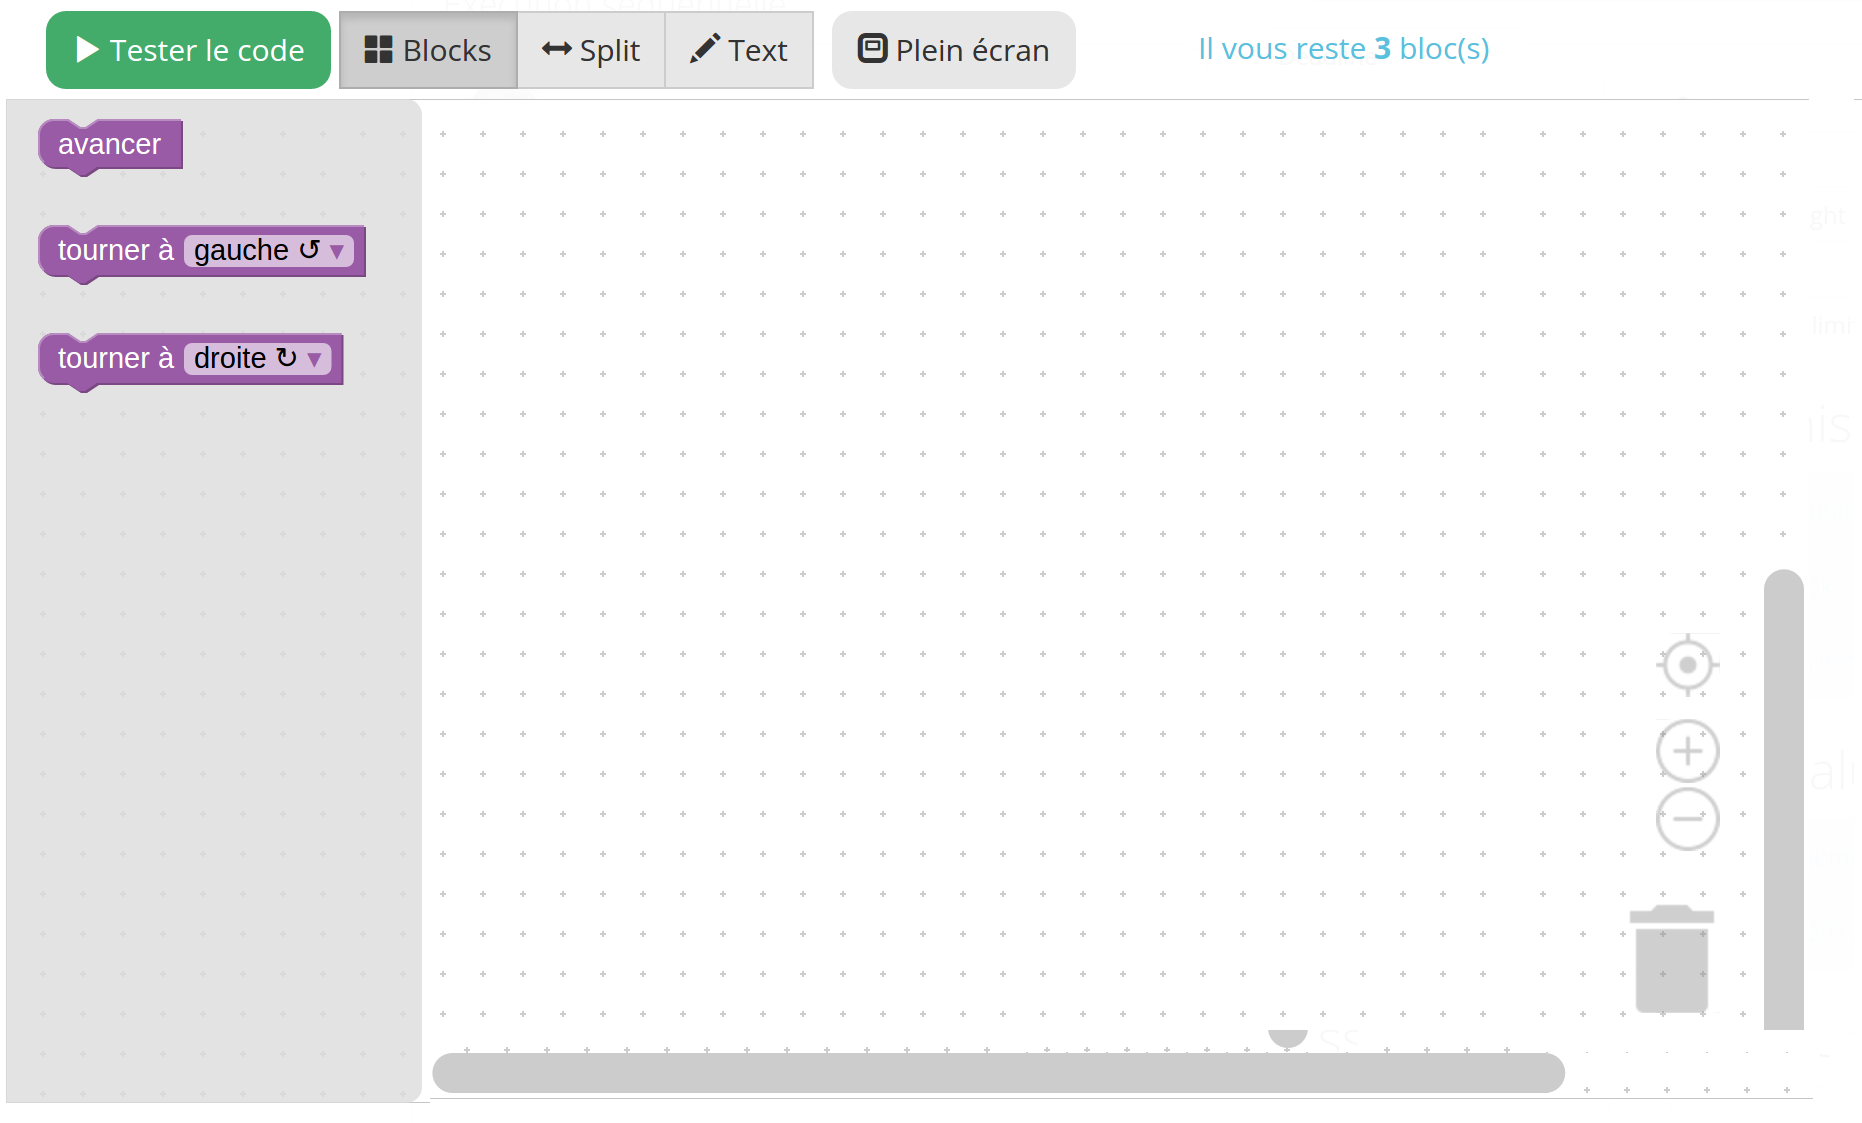
\includegraphics[width=\linewidth]{interface.png}
\end{frame}

\begin{frame}
	\frametitle{L'interface (La boite à outils)}

	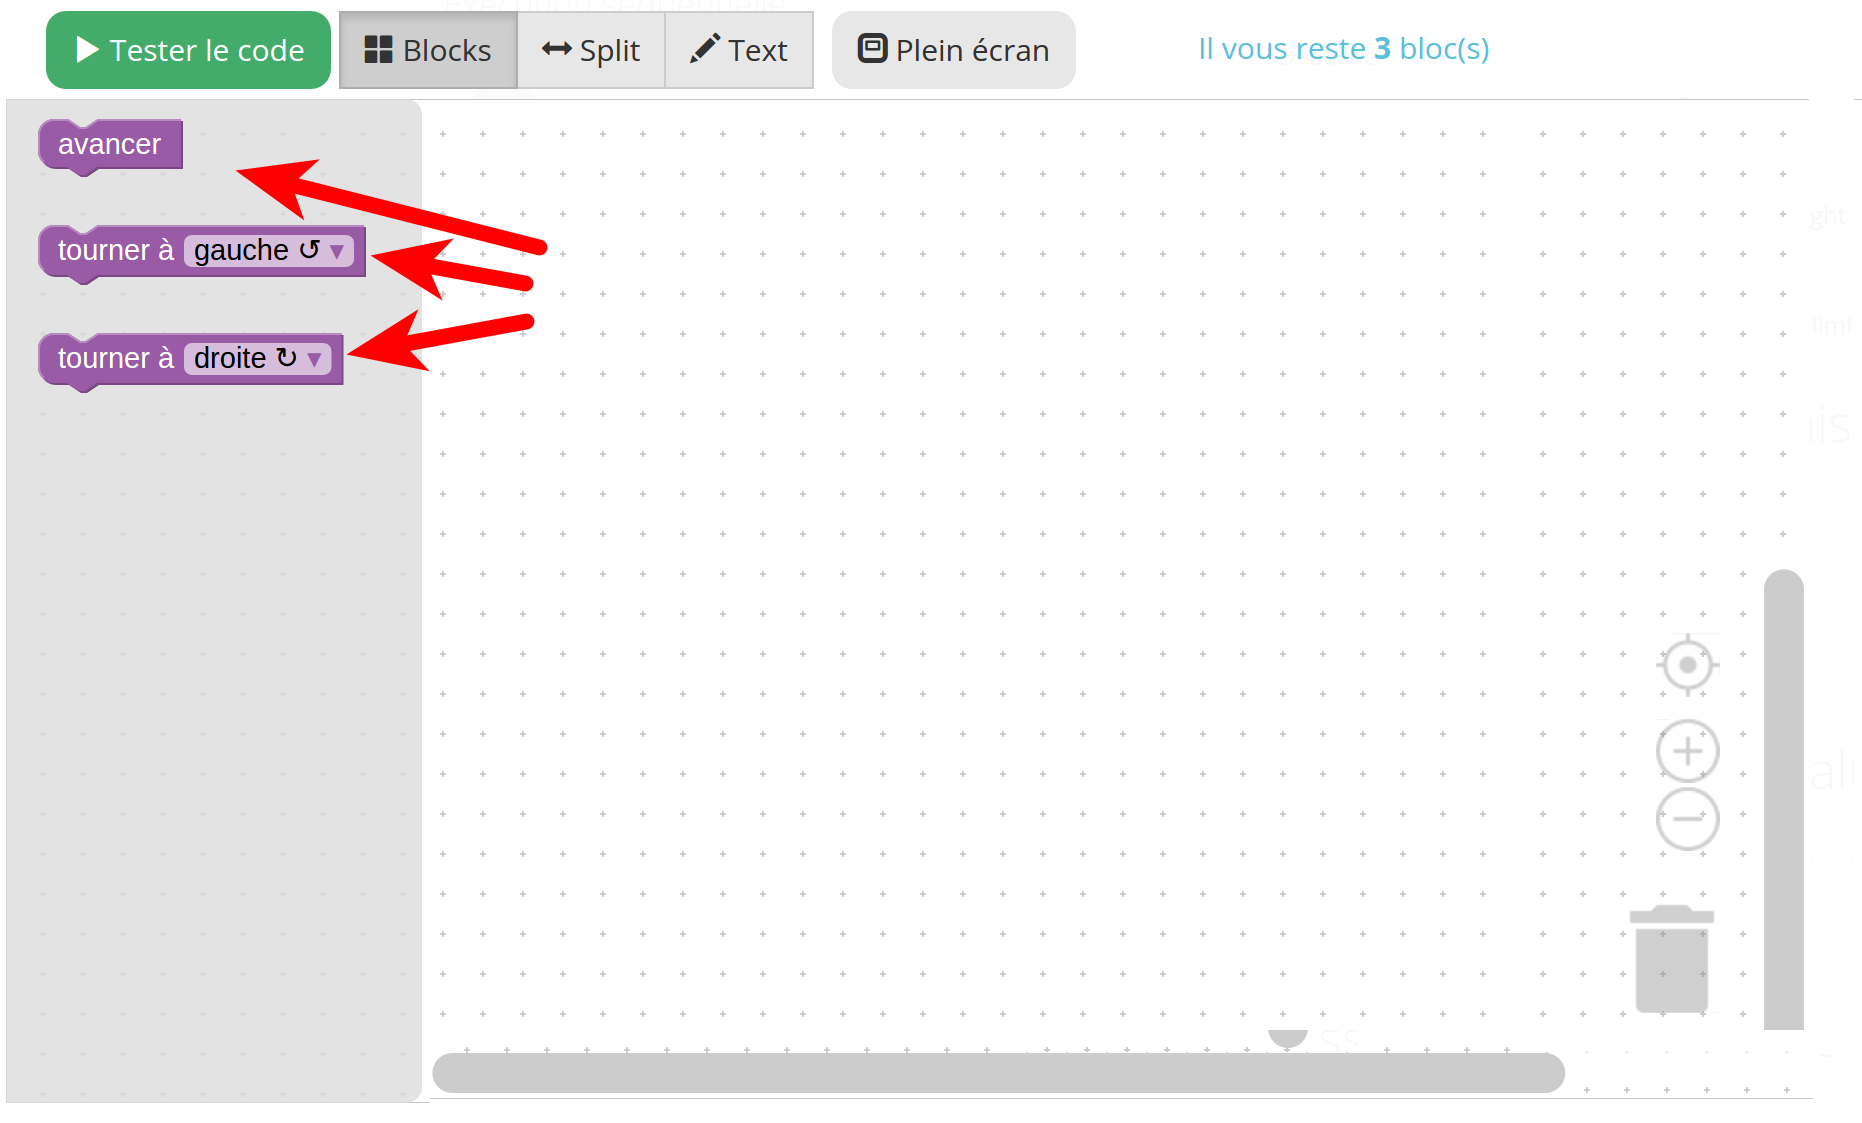
\includegraphics[width=\linewidth]{interface_toolbox.png}
\end{frame}

\begin{frame}
	\frametitle{L'interface (L'espace de travail)}

	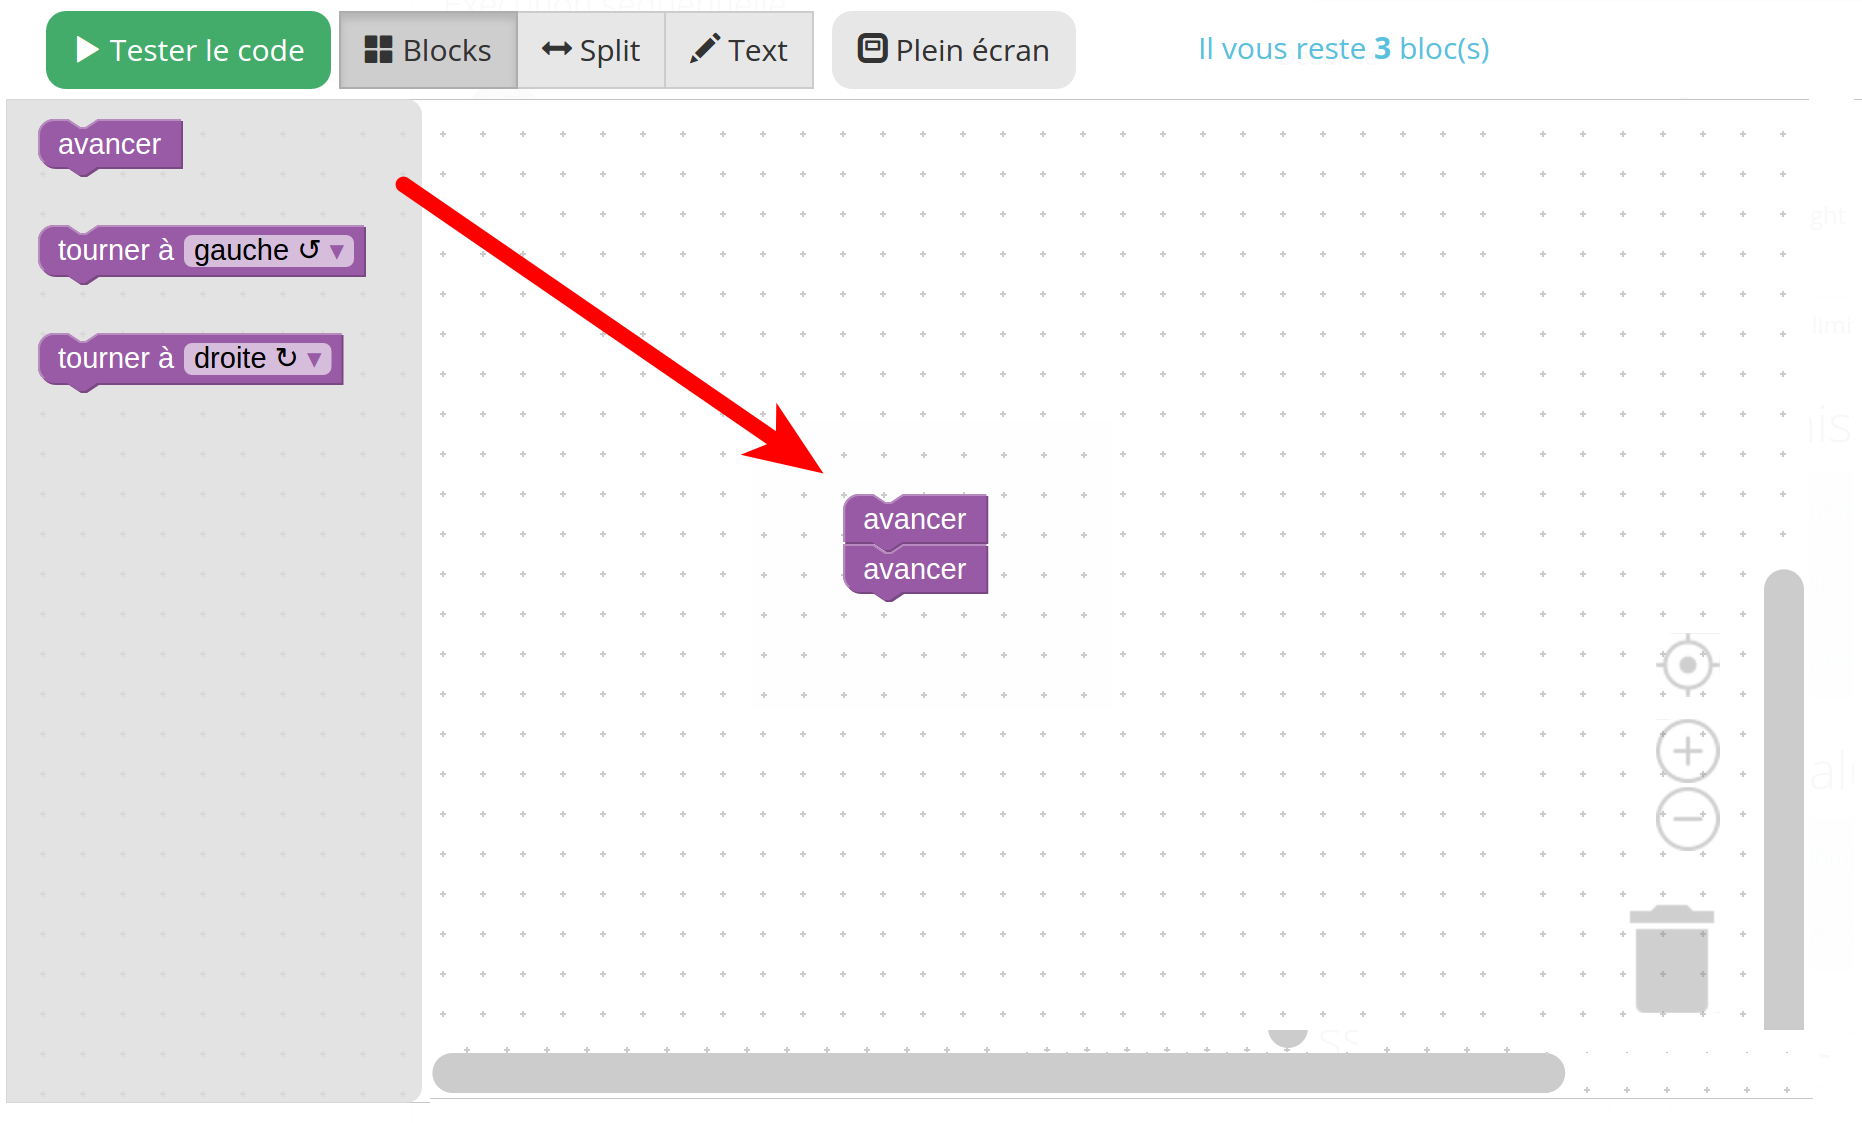
\includegraphics[width=\linewidth]{interface_workspace.png}
\end{frame}

\begin{frame}
	\frametitle{L'interface (Tester son code)}

	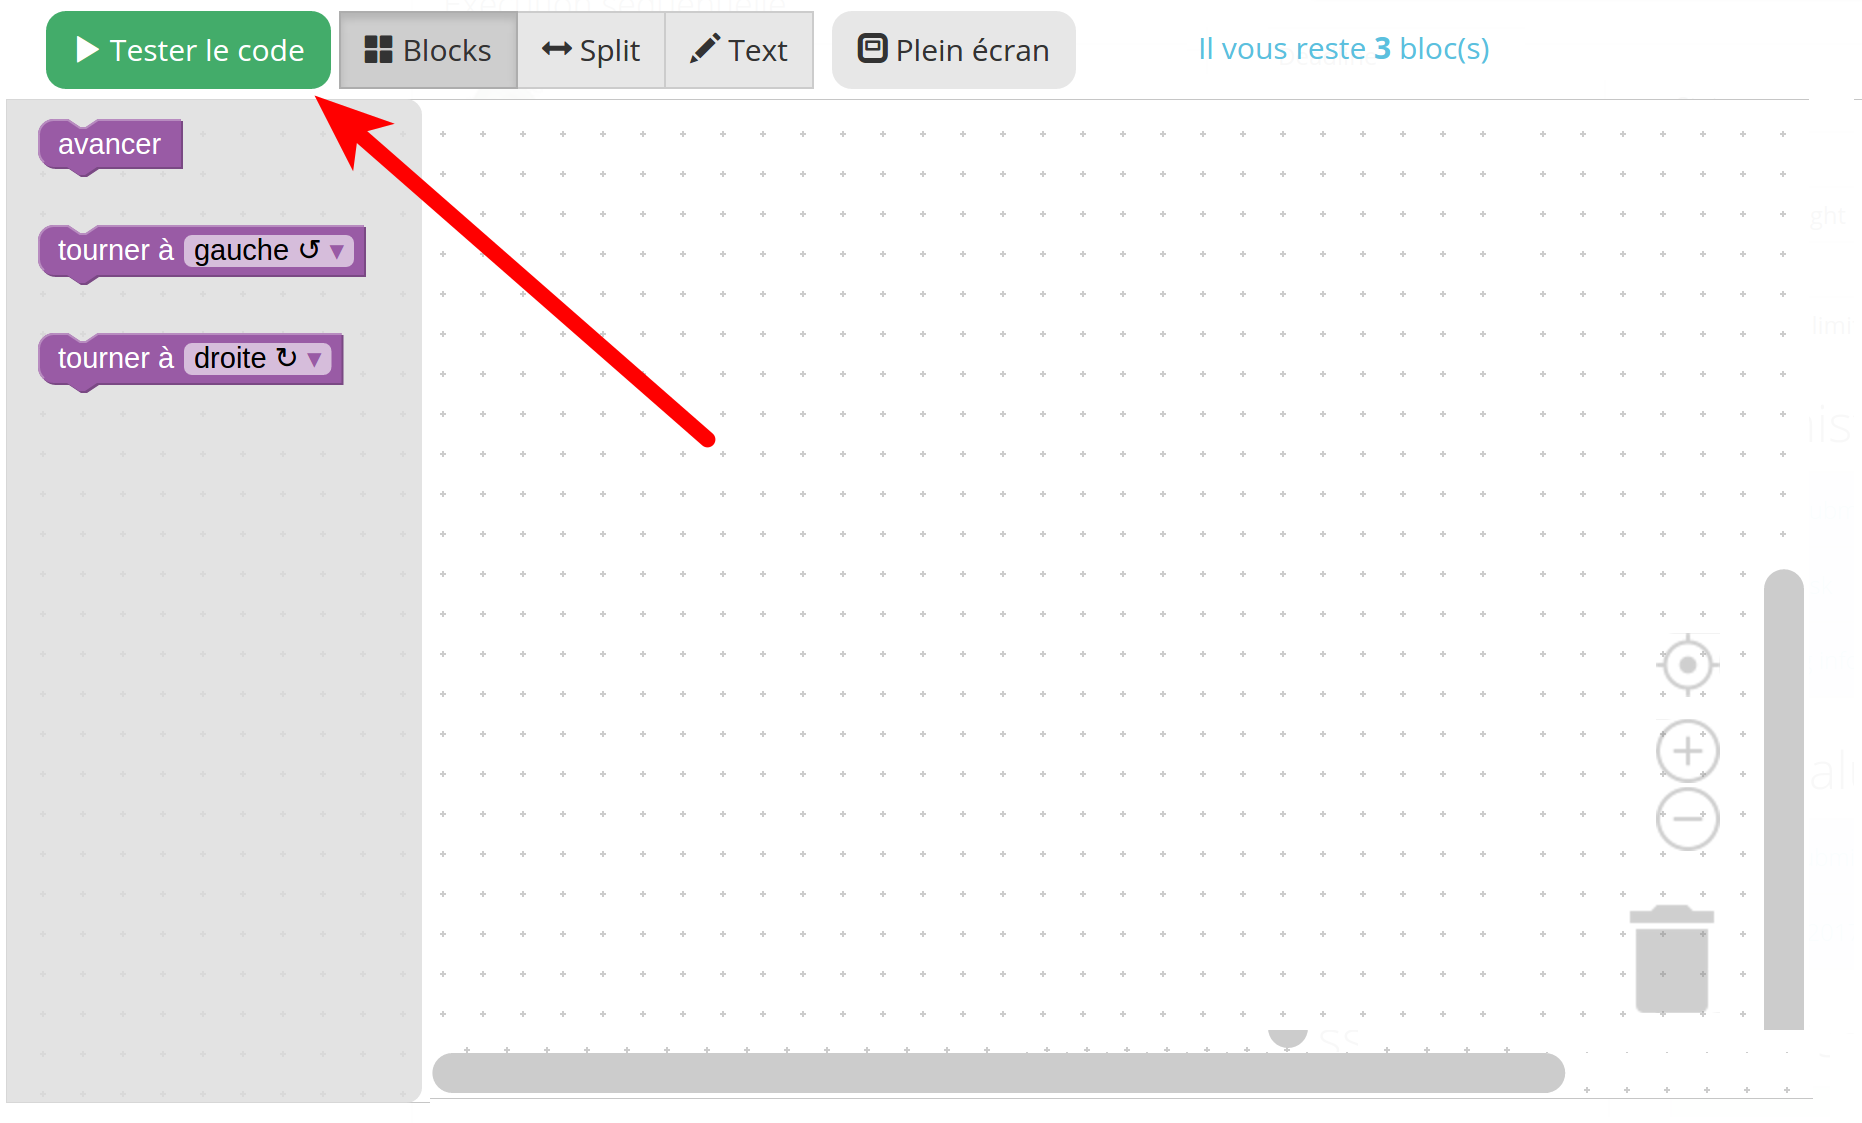
\includegraphics[width=\linewidth]{interface_codetest.png}
\end{frame}

\begin{frame}
	\frametitle{L'interface (La limite de blocs)}

	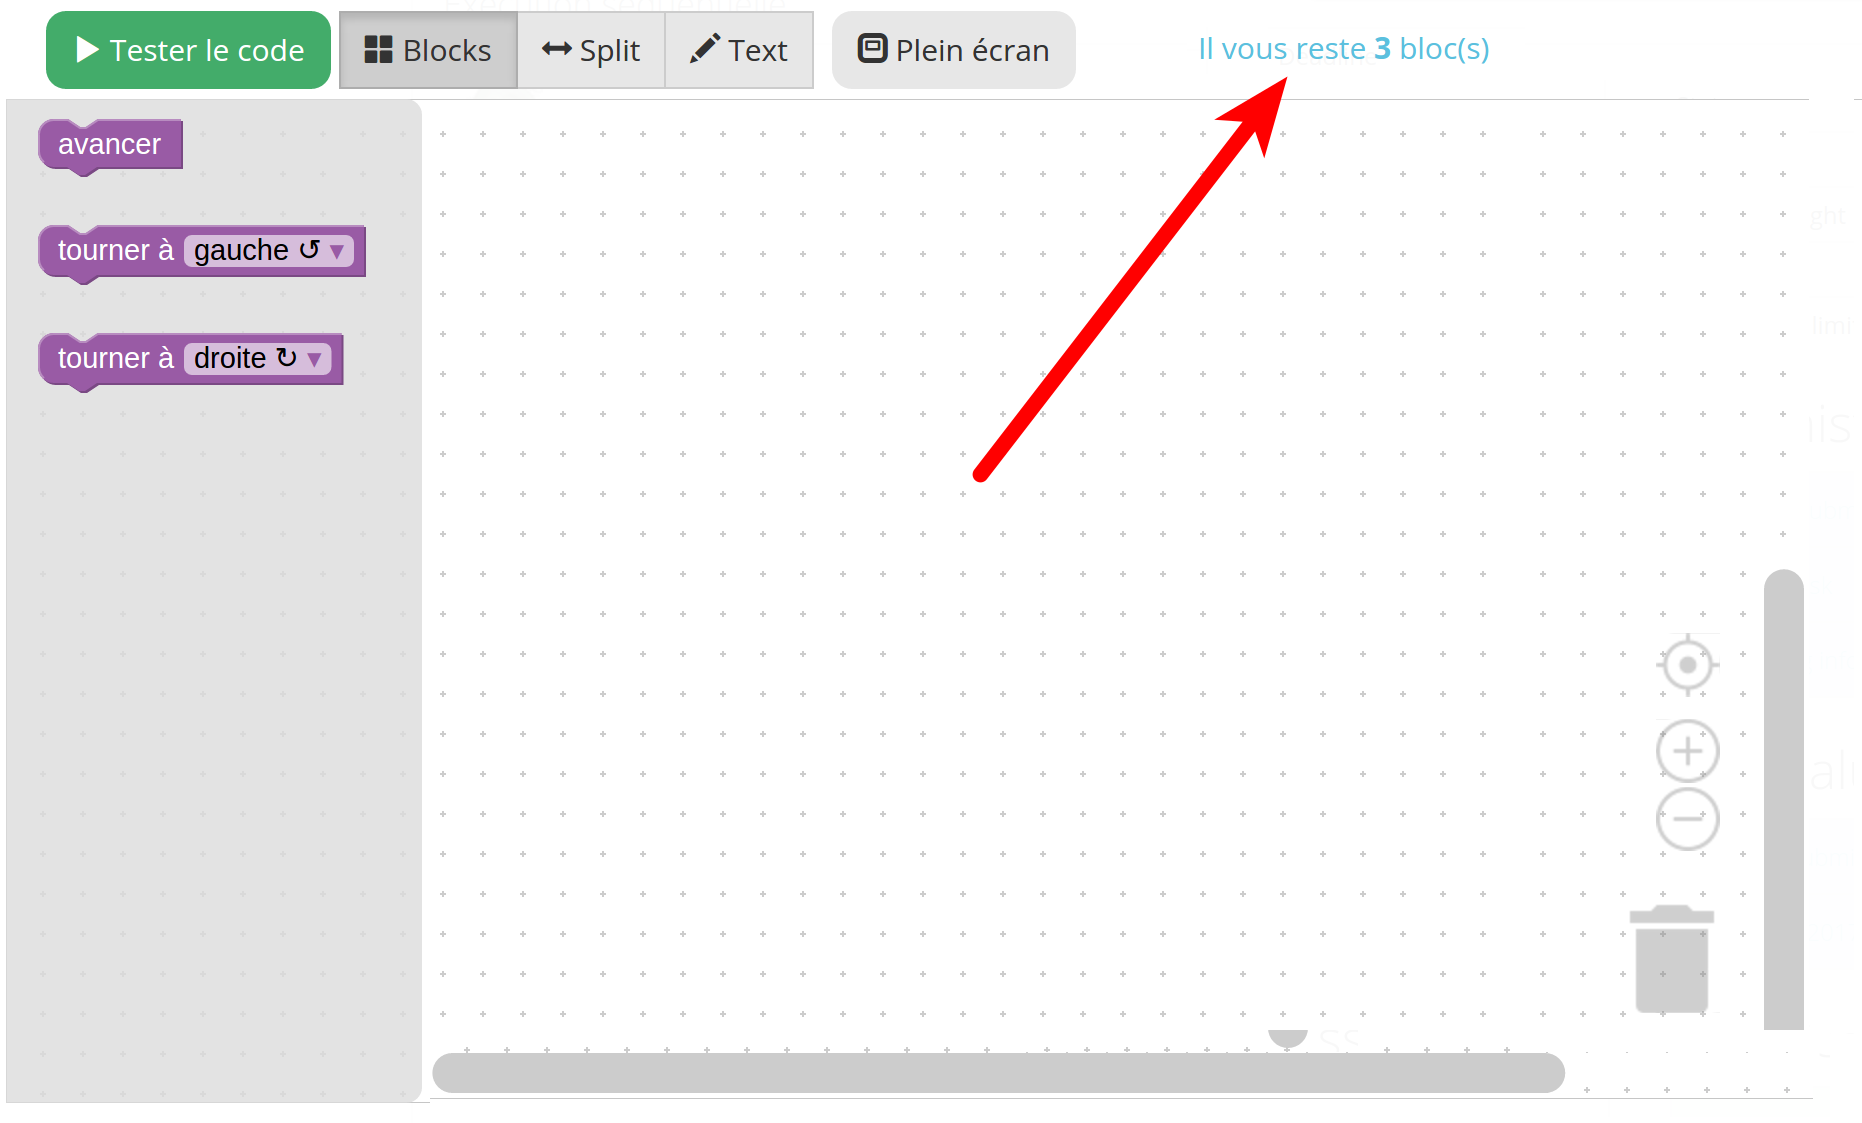
\includegraphics[width=\linewidth]{interface_blockslimit.png}
\end{frame}

\begin{frame}
	\frametitle{L'interface (Le plein écran)}

	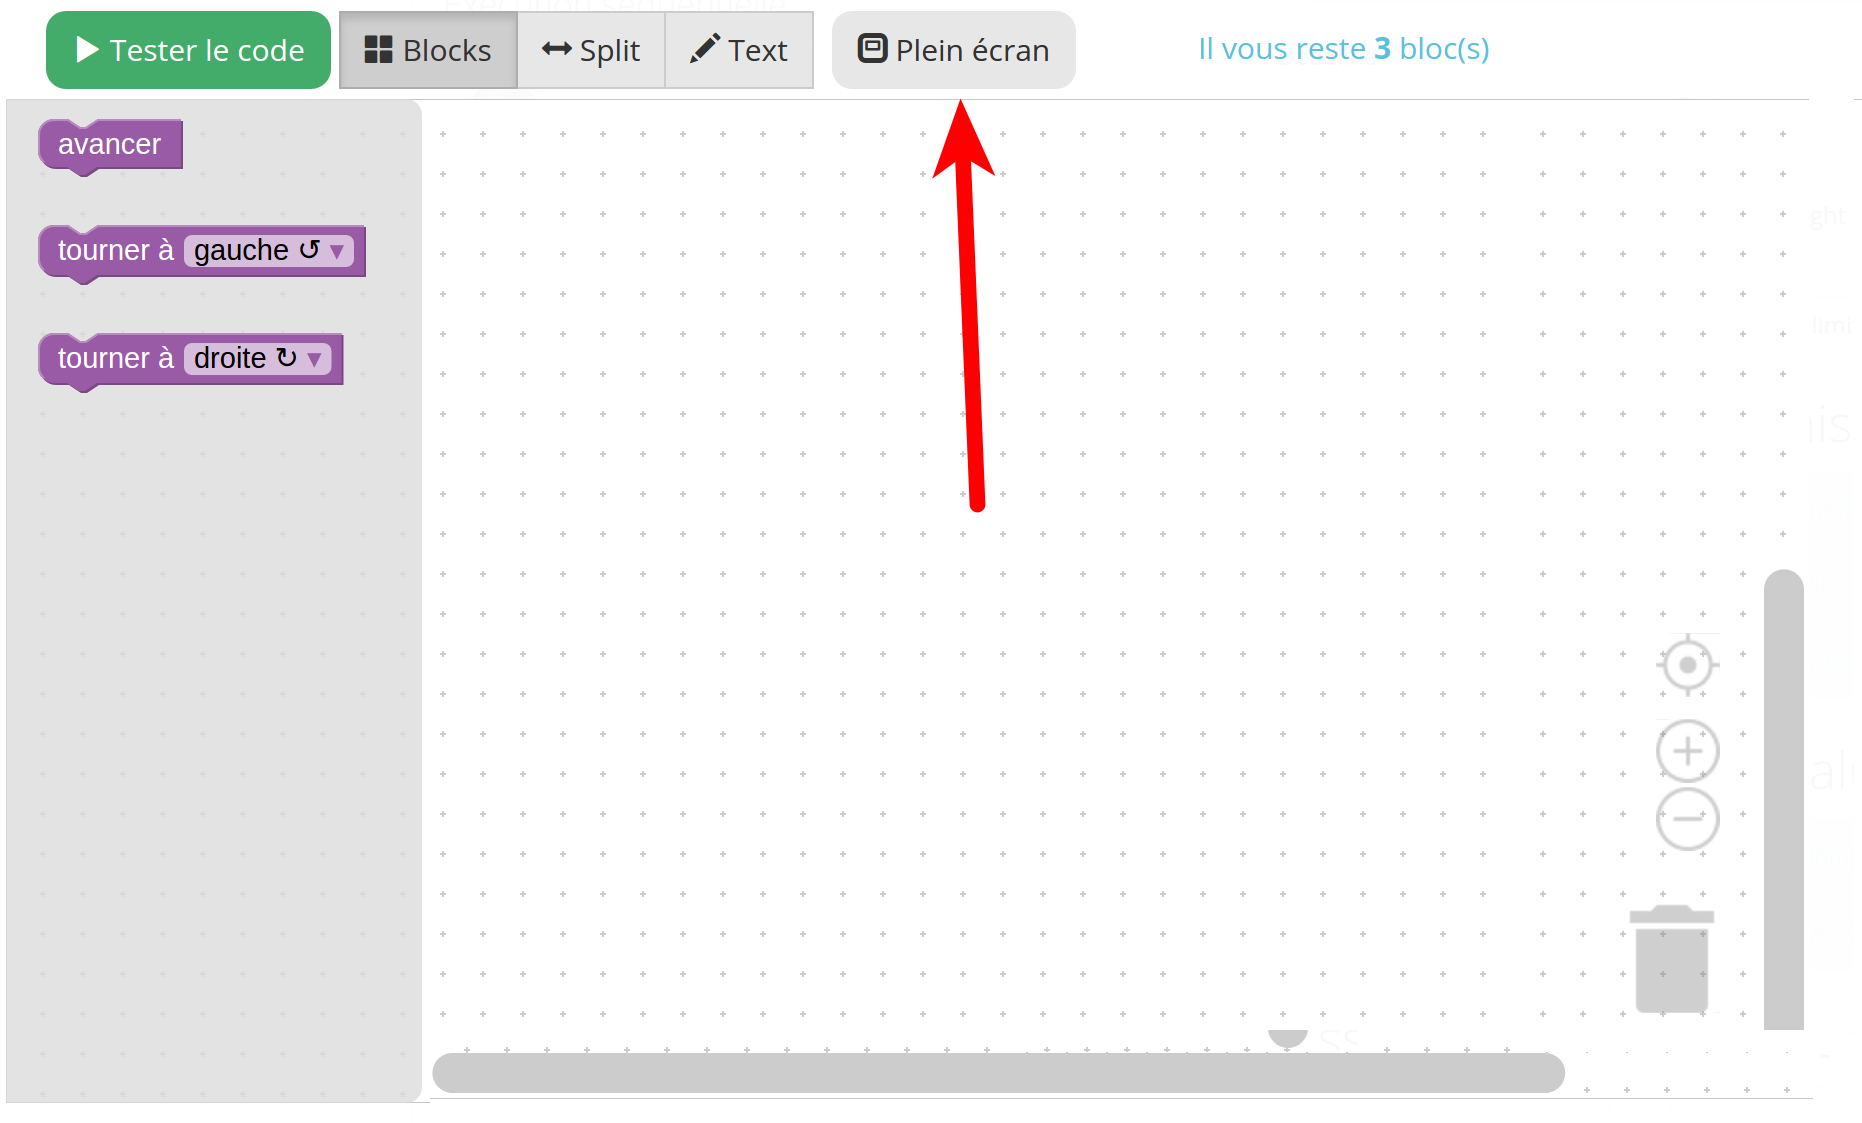
\includegraphics[width=\linewidth]{interface_fullscreen.png}
\end{frame}

\begin{frame}
	\frametitle{L'interface (La poubelle)}

	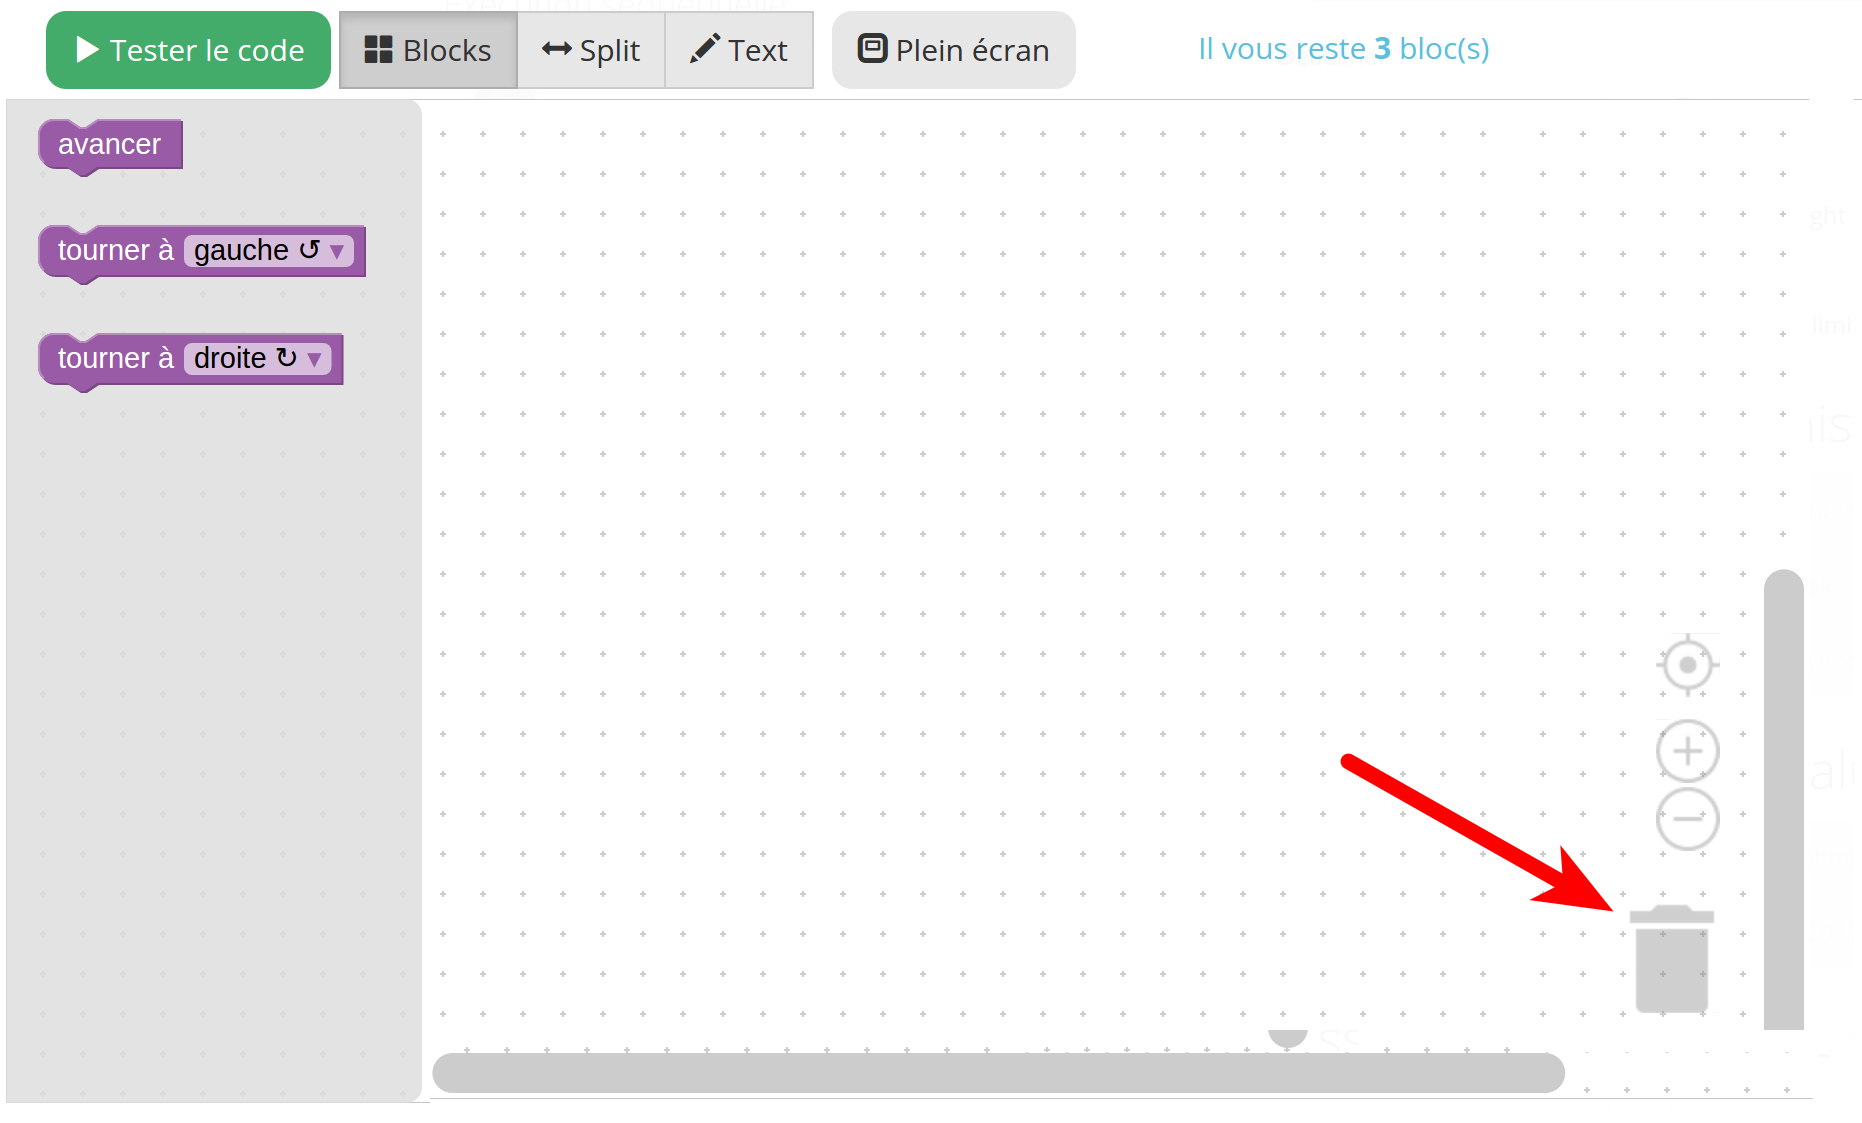
\includegraphics[width=\linewidth]{interface_trash.png}
\end{frame}

\begin{frame}
	\frametitle{La visualisation}

	\centering
	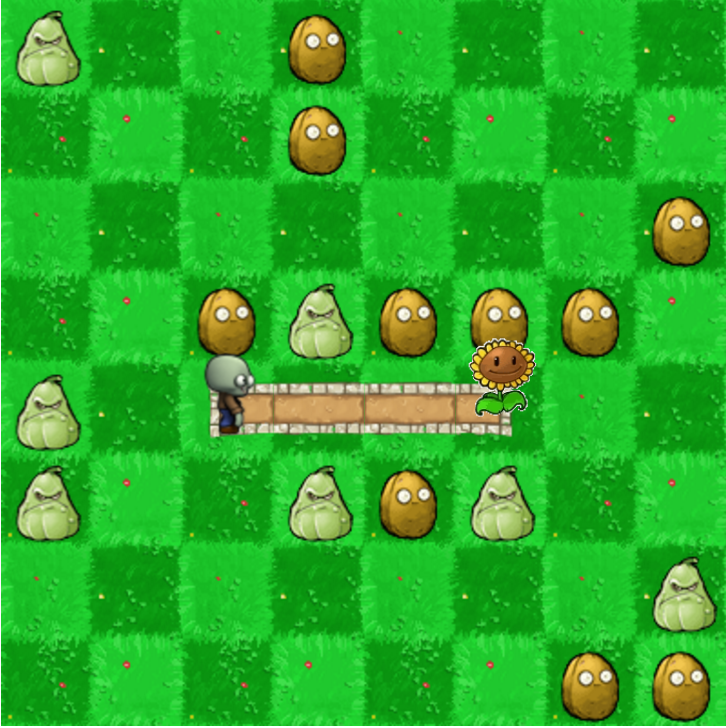
\includegraphics[width=0.65\linewidth]{visualisation_pvz.png}
\end{frame}

\section{Présentation des concepts}

\begin{frame}
	\frametitle{L'exécution séquentielle}

	Les blocs peuvent être empilés les uns en dessous des autres
	pour faire une \textbf{séquence d'instructions}.

	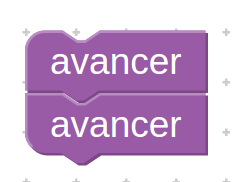
\includegraphics[width=0.45\linewidth]{blocks_2moveForward.png}
	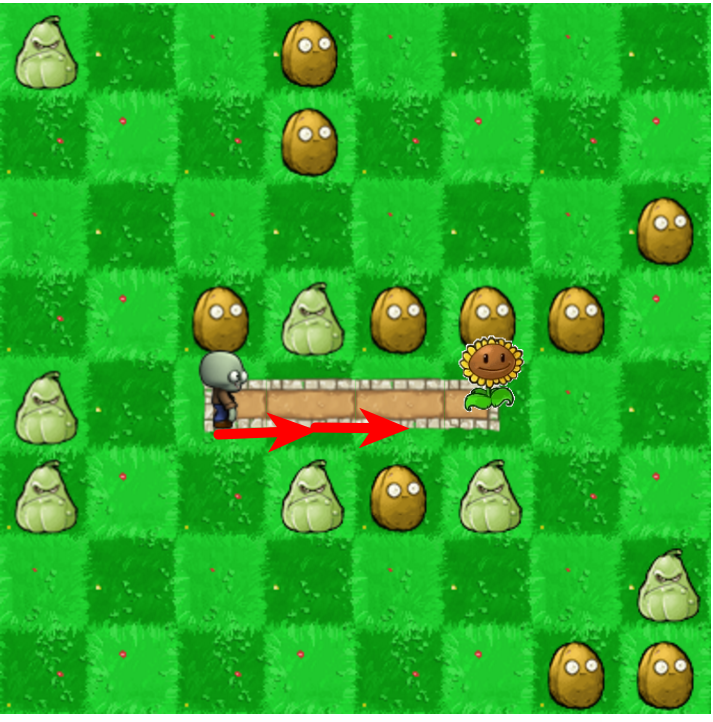
\includegraphics[width=0.45\linewidth]{visualization_2moveForward.png}

	L'instruction \enquote{avancer} fait avancer le personnage d'une case. En empilant
	deux blocs \enquote{avancer}, vous avancez de 2 cases.
\end{frame}

\begin{frame}
	\frametitle{Les conditions}

	Une \textbf{condition} vous permet de faire une action \textbf{si une propriété est vraie},
	ou autre chose si c'est faux.

	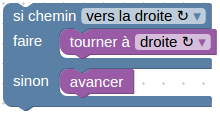
\includegraphics[width=0.45\linewidth]{blocks_ifElse.png}
	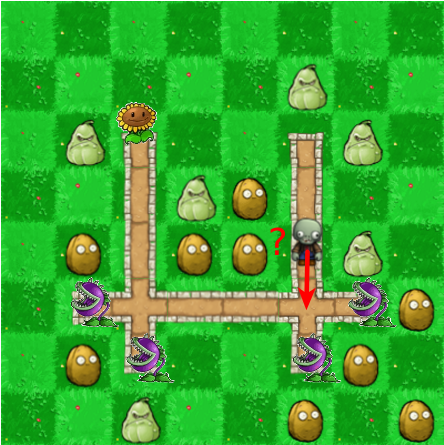
\includegraphics[width=0.45\linewidth]{vizualization_ifElse.png}

\end{frame}

\begin{frame}
	\frametitle{Les boucles}

	Il arrive que des actions doivent être faites de nombreuses fois. Les \textbf{boucles}
	permettent de \textbf{répéter} les actions un certain nombre de fois.

	\begin{center}
		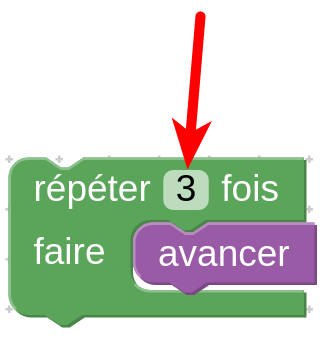
\includegraphics[width=0.45\linewidth]{blocks_forloop.png}
		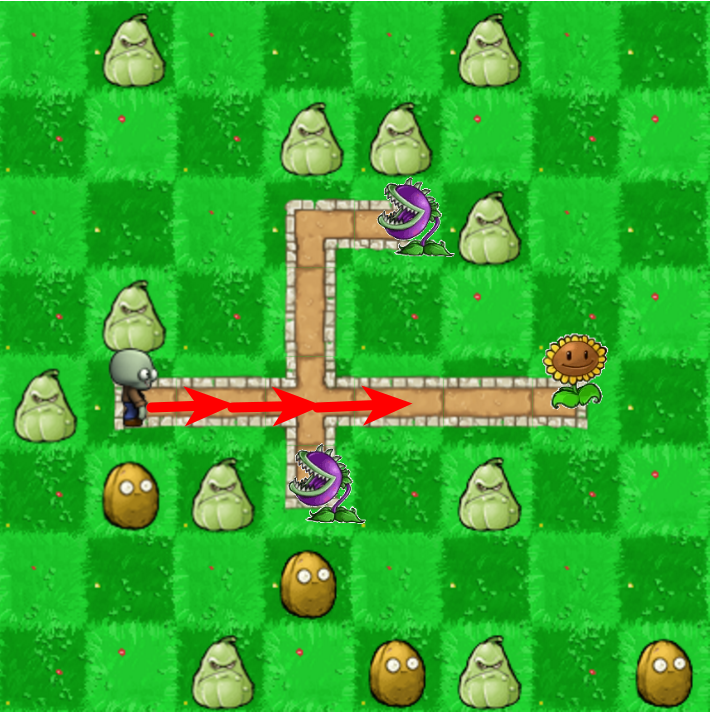
\includegraphics[width=0.45\linewidth]{visualization_forloop.png}
	\end{center}

	Vous pouvez changer le nombre de répétitions !
\end{frame}

\begin{frame}
	\frametitle{Les fonctions}

	Vous pouvez \textbf{nommer} une série d'actions. Ceci vous permet de \textit{résumer}
	une série d'actions avec une seule action.

	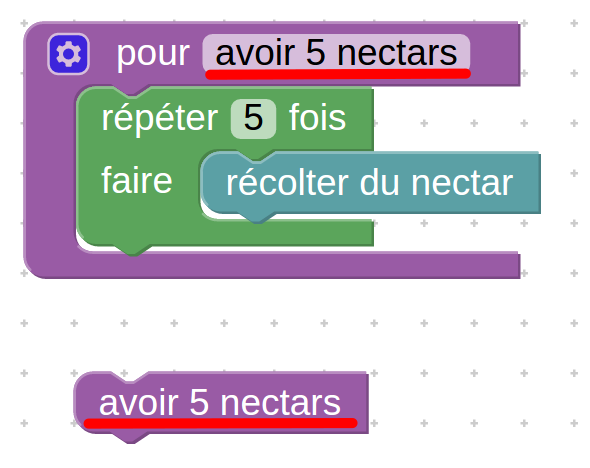
\includegraphics[width=0.45\linewidth]{blocks_function.png}
	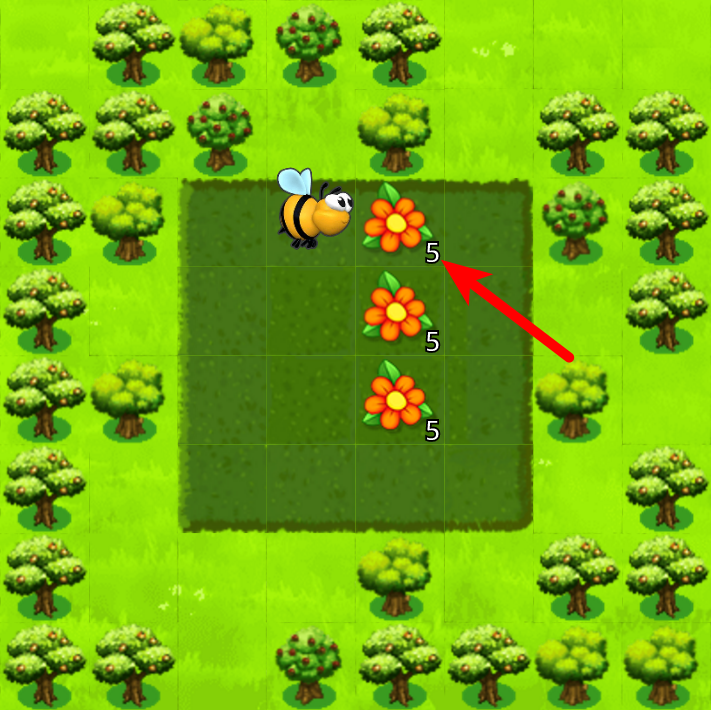
\includegraphics[width=0.45\linewidth]{vizualization_function.png}

	Avec un seul bloc \enquote{avoir 5 nectars}, vous effectuez en réalité une boucle !
\end{frame}

\begin{frame}
	\frametitle{A vous de jouer !}

	Vous pouvez \textbf{tester} votre code autant que vous voulez, faites-le !

	\begin{center}
		
\includegraphics[width=0.5\linewidth]{testcode.png}
	\end{center}

	Quand vous êtes satisfait de votre code, \textbf{enregistrez-le} pour confirmer
	votre réussite !

	\begin{center}
		
\includegraphics[width=\linewidth]{save.png}
	\end{center}
\end{frame}

\end{document}
